%====================================================================
%  第3章 复数  ——  3.3 复数的几何表示
%  高中数学课堂 PPT（Beamer + TikZ）
%  说明：本版本重新组织了教学顺序，加入了逐步动画（\pause）
%       修正了原文件中：重复的导言区设置、游离在 frame 外的内容、
%       过载的单页、缺失的首页容错等问题。
%====================================================================
\documentclass[aspectratio=169,UTF8,11pt]{ctexbeamer}

%==================== 宏包 ====================
\usepackage{amsmath,amssymb,bm}
% 字体：Times 风格（试卷感）
% 如果你的 TeX Live 有 newtxtext 宏包（完整版通常有），可以启用下面这行并注释掉 mathptmx
%\usepackage{newtxtext,newtxmath}
\usepackage{mathptmx}
\usepackage{graphicx}
\usepackage{tikz}
\usepackage[most]{tcolorbox}
\usepackage{array,booktabs,multirow}
\usepackage{multicol}
\usepackage{ragged2e}
\usepackage{xcolor}
\usepackage{pifont}
\usetikzlibrary{arrows.meta,calc,positioning,shapes.callouts,shapes.geometric,fit,backgrounds}

%==================== 颜色定义（统一） ====================
\definecolor{pptred}{RGB}{220,0,0}
\definecolor{pptblue}{RGB}{0,0,220}
\definecolor{pptline}{RGB}{0,155,235}
\definecolor{pptpink}{RGB}{239,214,219}
\definecolor{pptlightblue}{RGB}{233,245,255}
\definecolor{pptgray}{RGB}{90,90,90}
\definecolor{schoolgreen}{RGB}{10,166,72}     % 首页绿色
\definecolor{schoolorange}{RGB}{236,140,32}   % 首页橙色
\definecolor{titlegreen}{RGB}{0,102,102}      % 正文页标题条
\definecolor{textgray}{RGB}{70,70,70}

%==================== Beamer 外观 ====================
\setbeamertemplate{navigation symbols}{}
\setbeamertemplate{itemize item}{\color{pptblue}$\blacktriangleright$}
\setbeamertemplate{itemize subitem}{\color{pptblue}\textbullet}
\setbeamersize{text margin left=0.55cm,text margin right=0.55cm}
\setlength{\parskip}{0.25em}

\setbeamercolor{normal text}{fg=black,bg=white}
\setbeamerfont{normal text}{size=\fontsize{14}{18}}

% 页脚：仅显示页码（极简风格）
\setbeamertemplate{footline}[frame number]

%==================== 自定义命令 ====================
% 章节标题：左侧绿色竖条 + 淡色背景条（替代原方框样式）
\newcommand{\SectionTitle}[1]{%
  \begin{tikzpicture}
    \node[
      anchor=west,
      inner sep=4pt,
      text width=\dimexpr\linewidth-16pt\relax,
      fill=titlegreen!8,
      font=\sffamily\bfseries\fontsize{17}{21}\selectfont
    ]
    (title) {\hspace{6pt}\color{titlegreen}#1};
    \fill[titlegreen] (title.south west) rectangle ++(4pt,\dimexpr\ht\strutbox+\dp\strutbox+16pt\relax);
  \end{tikzpicture}\par\vspace{0.1cm}
}

% 蓝色小标题：适用于二级标题
\newcommand{\BlueTitle}[1]{%
  {\color{pptblue}\sffamily\bfseries\fontsize{18}{22}\selectfont
   \raisebox{1pt}{\rule{3pt}{14pt}}\ #1\par}\vspace{0.1cm}
}

% 保留原 BlackBoxTitle 作为别名，兼容已有调用（直接转为 SectionTitle）
\newcommand{\BlackBoxTitle}[1]{\SectionTitle{#1}}

% 统一页标题：采用“类比联想，探究新知”页的标题风格
\newcommand{\TopPageTitle}[1]{%
  \begin{tikzpicture}
    \fill[schoolgreen] (0,0) rectangle (0.4,0.4);
    \fill[schoolgreen!60] (0.5,-0.12) rectangle (0.82,0.2);
    \node[anchor=west,font=\bfseries\fontsize{19}{23}\selectfont,text=schoolgreen]
      at (1.1,0.18) {#1};
  \end{tikzpicture}\par\vspace{0.35cm}
}

\newcommand{\ExampleTag}[1]{%
  {\color{pptblue}\sffamily\bfseries\fontsize{17}{21}\selectfont 例#1}\quad
}

\newtcolorbox{calloutbox}[1][]{
  enhanced,colback=pptlightblue,colframe=pptblue,
  boxrule=0.5pt,arc=2mm,
  left=2mm,right=2mm,top=1mm,bottom=1mm,#1
}

\newtcolorbox{pinknote}[1][]{
  enhanced,colback=pptpink,colframe=black!70,
  boxrule=0.5pt,arc=3mm,
  left=2mm,right=2mm,top=1mm,bottom=1mm,#1
}

\newtcolorbox{keybox}[1][]{
  enhanced,colback=yellow!15,colframe=orange!70!black,
  boxrule=0.6pt,arc=2mm,
  left=2mm,right=2mm,top=1mm,bottom=1mm,#1
}

\newcommand{\modz}[1]{\left\lvert #1 \right\rvert}

%==================== TikZ 图形命令 ====================

% 实轴向量图（问题引入）
\newcommand{\RealAxisVectorTikz}{%
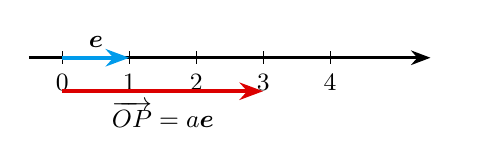
\begin{tikzpicture}[x=0.85cm,y=0.85cm,>=Stealth]
  \draw[->,line width=0.9pt] (-0.5,0)--(5.5,0) node[right]{};
  \foreach \x in {0,1,2,3,4}
    \draw (\x,0.1)--(\x,-0.1) node[below]{\small $\x$};
  \draw[pptline,line width=1.6pt,-{Stealth[length=3mm,width=2.2mm]}] (0,0)--(1,0);
  \node[above] at (0.5,0) {\small $\bm{e}$};
  \draw[pptred,line width=1.6pt,-{Stealth[length=3mm,width=2.2mm]}] (0,-0.5)--(3,-0.5);
  \node[below] at (1.5,-0.5) {\small $\overrightarrow{OP}=a\bm{e}$};
\end{tikzpicture}}

% 复平面点表示
\newcommand{\ComplexPointFigure}{%
\begin{tikzpicture}[x=0.85cm,y=0.85cm,>=Stealth]
  \draw[->,line width=0.9pt] (-0.3,0)--(4.6,0) node[below]{$x$};
  \draw[->,line width=0.9pt] (0,-0.3)--(0,4.4) node[left]{$y$};
  \coordinate (Z) at (3.2,2.8);
  \draw[densely dashed] (0,2.8)--(Z)--(3.2,0);
  \fill (Z) circle (1.5pt) node[above right=-1pt]{$Z(a,b)$};
  \node[below left] at (0,0) {$O$};
  \node[below] at (3.2,0) {$a$};
  \node[left] at (0,2.8) {$b$};
\end{tikzpicture}}

% 复平面 + 实轴 + 虚轴 标注
\newcommand{\ComplexPlaneCalloutFigure}{%
\begin{tikzpicture}[x=0.7cm,y=0.7cm,>=Stealth]
  \draw[->,line width=0.9pt] (-4.2,0)--(4.3,0) node[below right]{$x$};
  \draw[->,line width=0.9pt] (0,-3.1)--(0,3.4) node[above right=-2pt]{$y$};
  \coordinate (Z) at (2.6,2.2);
  \draw[densely dashed] (0,2.2)--(Z)--(2.6,0);
  \draw[->,line width=0.9pt] (0,0)--(Z);
  \fill (Z) circle (1.4pt) node[above right=-1pt]{$Z(a,b)$};
  \node[below left] at (0,0) {$O$};
  \node[below] at (2.6,0) {$a$};
  \node[left] at (0,2.2) {$b$};
  \node[draw,ellipse,minimum width=2.5cm,minimum height=0.9cm,fill=pptlightblue] (cp) at (0,4.2) {\small 复平面};
  \draw[line width=0.6pt] (cp.south) -- (1.5,3.0);
  \node[draw,ellipse,minimum width=1.5cm,minimum height=0.8cm,fill=pptlightblue] (rx) at (-3.2,1.5) {\small 实轴};
  \draw[line width=0.6pt] (rx.south east) -- (-1.8,0.05);
  \node[draw,ellipse,minimum width=1.5cm,minimum height=0.8cm,fill=pptlightblue] (ix) at (3.3,-2.3) {\small 虚轴};
  \draw[line width=0.6pt] (ix.west) -- (0.15,-1.3);
\end{tikzpicture}}

% 复数的向量表示
\newcommand{\ComplexVectorFigure}{%
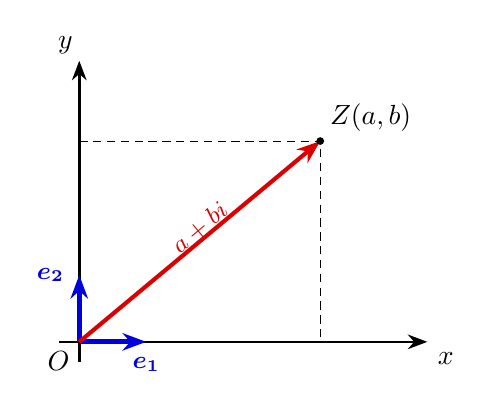
\begin{tikzpicture}[x=0.85cm,y=0.85cm,>=Stealth]
  \draw[->,line width=0.9pt] (-0.3,0)--(5.2,0) node[below right]{$x$};
  \draw[->,line width=0.9pt] (0,-0.3)--(0,4.2) node[above left=-2pt]{$y$};
  \coordinate (P) at (3.6,3.0);
  \draw[densely dashed] (0,3.0)--(P)--(3.6,0);
  % 基向量 e1, e2
  \draw[pptblue,line width=1.8pt,-{Stealth[length=3mm,width=2.2mm]}] (0,0)--(1,0);
  \draw[pptblue,line width=1.8pt,-{Stealth[length=3mm,width=2.2mm]}] (0,0)--(0,1);
  \draw[pptred,line width=1.5pt,-{Stealth[length=3mm,width=2.2mm]}] (0,0)--(P);
  \node[below left] at (0,0) {$O$};
  \node[below=2pt,text=pptblue] at (1,0) {\small $\bm{e_1}$};
  \node[left=2pt,text=pptblue] at (0,1) {\small $\bm{e_2}$};
  \fill (P) circle (1.4pt);
  \node[above right] at (P) {$Z(a,b)$};
  \node[rotate=40,text=pptred] at (1.8,1.7) {\small $a+bi$};
\end{tikzpicture}}

% 三者对应关系图
\newcommand{\ComplexCorrespondenceFigure}{%
\begin{tikzpicture}[x=0.9cm,y=0.9cm,>=Stealth]
  \node[draw,rounded corners,fill=pptlightblue,minimum width=3.5cm,minimum height=1.2cm,align=center] (top) at (0,2.3) {复数\\ $z=a+bi$};
  \node[draw,rounded corners,fill=pptlightblue,minimum width=3.5cm,minimum height=1.2cm,align=center] (left) at (-3.8,-1) {复平面内的\\ 点 $Z(a,b)$};
  \node[draw,rounded corners,fill=pptlightblue,minimum width=3.5cm,minimum height=1.2cm,align=center] (right) at (3.8,-1) {平面向量\\ $\overrightarrow{OZ}$};
  \draw[<->,line width=1pt,pptblue] (top.225)--(left.45) node[midway,above left=-2pt]{\small 一一对应};
  \draw[<->,line width=1pt,pptblue] (top.315)--(right.135) node[midway,above right=-2pt]{\small 一一对应};
  \draw[<->,line width=1pt,pptblue] (left.east)--(right.west) node[midway,below]{\small 一一对应};
\end{tikzpicture}}

% 例1：四个点
\newcommand{\ExampleOneFigure}{%
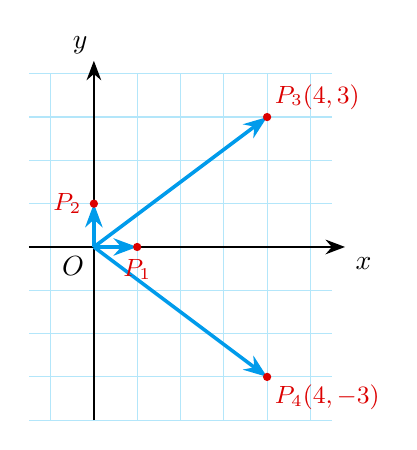
\begin{tikzpicture}[x=0.55cm,y=0.55cm,>=Stealth]
  \draw[step=1,draw=cyan!30,line width=0.4pt] (-1.5,-4) grid (5.5,4);
  \draw[->,line width=0.9pt] (-1.5,0)--(5.8,0) node[below right]{$x$};
  \draw[->,line width=0.9pt] (0,-4)--(0,4.3) node[above left=-2pt]{$y$};
  \coordinate (P1) at (1,0); \coordinate (P2) at (0,1);
  \coordinate (P3) at (4,3); \coordinate (P4) at (4,-3);
  \draw[pptline,line width=1.3pt,-{Stealth[length=3mm,width=2.2mm]}] (0,0)--(P1);
  \draw[pptline,line width=1.3pt,-{Stealth[length=3mm,width=2.2mm]}] (0,0)--(P2);
  \draw[pptline,line width=1.3pt,-{Stealth[length=3mm,width=2.2mm]}] (0,0)--(P3);
  \draw[pptline,line width=1.3pt,-{Stealth[length=3mm,width=2.2mm]}] (0,0)--(P4);
  \fill[pptred] (P1) circle (1.5pt) node[below=1pt]{\small $P_1$};
  \fill[pptred] (P2) circle (1.5pt) node[left=1pt]{\small $P_2$};
  \fill[pptred] (P3) circle (1.5pt) node[above right=-1pt]{\small $P_3(4,3)$};
  \fill[pptred] (P4) circle (1.5pt) node[below right=-1pt]{\small $P_4(4,-3)$};
  \node[below left] at (0,0) {$O$};
\end{tikzpicture}}

% 例2：圆环
\newcommand{\AnnulusFigure}{%
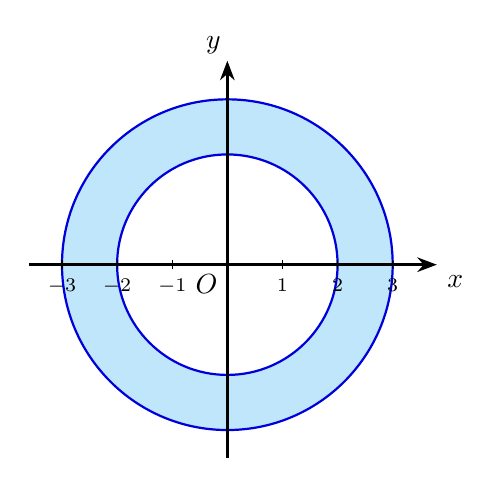
\begin{tikzpicture}[x=0.7cm,y=0.7cm,>=Stealth]
  \fill[pptline!25,even odd rule] (0,0) circle (3) (0,0) circle (2);
  \draw[pptblue,thick] (0,0) circle (2);
  \draw[pptblue,thick] (0,0) circle (3);
  \draw[->,line width=0.9pt] (-3.6,0)--(3.8,0) node[below right]{$x$};
  \draw[->,line width=0.9pt] (0,-3.5)--(0,3.7) node[above left=-2pt]{$y$};
  \foreach \x in {-3,-2,-1,1,2,3}
    \draw (\x,0.08)--(\x,-0.08) node[below]{\scriptsize $\x$};
  \node[below left] at (0,0) {$O$};
\end{tikzpicture}}

% 共轭复数图
\newcommand{\ConjugateGridFigure}{%
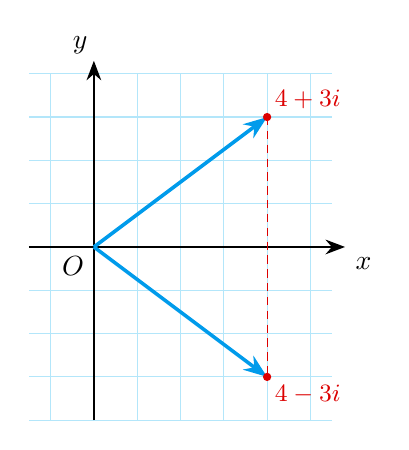
\begin{tikzpicture}[x=0.55cm,y=0.55cm,>=Stealth]
  \draw[step=1,draw=cyan!30,line width=0.4pt] (-1.5,-4) grid (5.5,4);
  \draw[->,line width=0.9pt] (-1.5,0)--(5.8,0) node[below right]{$x$};
  \draw[->,line width=0.9pt] (0,-4)--(0,4.3) node[above left=-2pt]{$y$};
  \coordinate (P3) at (4,3); \coordinate (P4) at (4,-3);
  \draw[pptline,line width=1.3pt,-{Stealth[length=3mm,width=2.2mm]}] (0,0)--(P3);
  \draw[pptline,line width=1.3pt,-{Stealth[length=3mm,width=2.2mm]}] (0,0)--(P4);
  \draw[densely dashed,pptred] (4,3)--(4,-3);
  \fill[pptred] (P3) circle (1.5pt) node[above right=-1pt]{\small $4+3i$};
  \fill[pptred] (P4) circle (1.5pt) node[below right=-1pt]{\small $4-3i$};
  \node[below left] at (0,0) {$O$};
\end{tikzpicture}}

% 加法几何意义：平行四边形
\newcommand{\AdditionFigure}{%
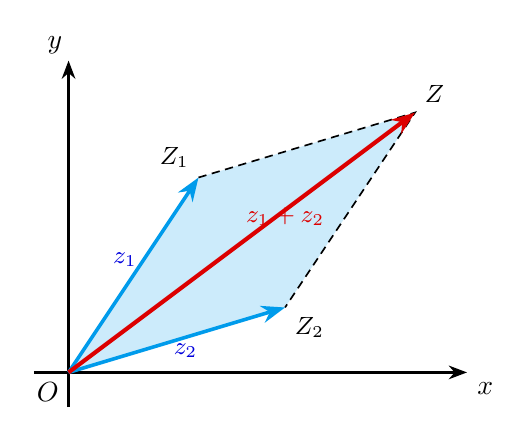
\begin{tikzpicture}[x=0.55cm,y=0.55cm,>=Stealth]
  \coordinate (O) at (0,0);
  \coordinate (Z1) at (3,4.5);
  \coordinate (Z2) at (5,1.5);
  \coordinate (Z)  at (8,6);
  \fill[pptline!20] (O)--(Z1)--(Z)--(Z2)--cycle;
  \draw[->,line width=0.8pt] (-0.8,0)--(9.2,0) node[below right]{$x$};
  \draw[->,line width=0.8pt] (0,-0.8)--(0,7.2) node[above left=-2pt]{$y$};
  \draw[densely dashed,line width=0.6pt] (Z1)--(Z)--(Z2);
  \draw[pptline,line width=1.3pt,-{Stealth[length=3mm,width=2.2mm]}] (O)--(Z1);
  \draw[pptline,line width=1.3pt,-{Stealth[length=3mm,width=2.2mm]}] (O)--(Z2);
  \draw[pptred,line width=1.5pt,-{Stealth[length=3mm,width=2.2mm]}] (O)--(Z);
  \node[below left] at (O) {$O$};
  \node[above left] at (Z1) {\small $Z_1$};
  \node[below right] at (Z2) {\small $Z_2$};
  \node[above right] at (Z) {\small $Z$};
  \node[pptblue] at (1.3,2.6) {\small $z_1$};
  \node[pptblue] at (2.7,0.5) {\small $z_2$};
  \node[pptred] at (5,3.6) {\small $z_1+z_2$};
\end{tikzpicture}}

% 减法几何意义
\newcommand{\SubtractionFigure}{%
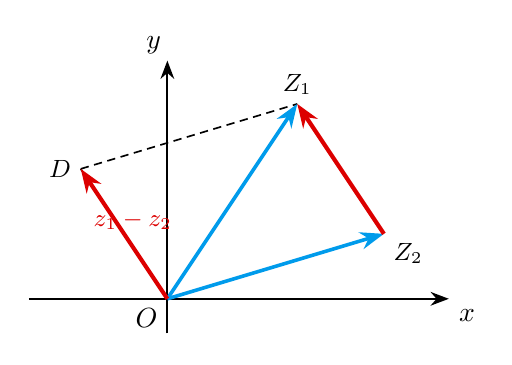
\begin{tikzpicture}[x=0.55cm,y=0.55cm,>=Stealth]
  \coordinate (O) at (0,0);
  \coordinate (Z1) at (3,4.5);
  \coordinate (Z2) at (5,1.5);
  \coordinate (D)  at (-2,3);
  \draw[->,line width=0.8pt] (-3.2,0)--(6.5,0) node[below right]{$x$};
  \draw[->,line width=0.8pt] (0,-0.8)--(0,5.5) node[above left=-2pt]{$y$};
  \draw[densely dashed,line width=0.6pt] (D)--(Z1);
  \draw[densely dashed,line width=0.6pt] (D)--(O);
  \draw[pptline,line width=1.3pt,-{Stealth[length=3mm,width=2.2mm]}] (O)--(Z1);
  \draw[pptline,line width=1.3pt,-{Stealth[length=3mm,width=2.2mm]}] (O)--(Z2);
  \draw[pptred,line width=1.5pt,-{Stealth[length=3mm,width=2.2mm]}] (O)--(D);
  \draw[pptred,line width=1.5pt,-{Stealth[length=3mm,width=2.2mm]}] (Z2)--(Z1);
  \node[below left] at (O) {$O$};
  \node[above] at (Z1) {\small $Z_1$};
  \node[below right] at (Z2) {\small $Z_2$};
  \node[left] at (D) {\small $D$};
  \node[pptred] at (-0.8,1.8) {\small $z_1-z_2$};
\end{tikzpicture}}

% 数乘几何意义
\newcommand{\ScalarMulFigure}{%
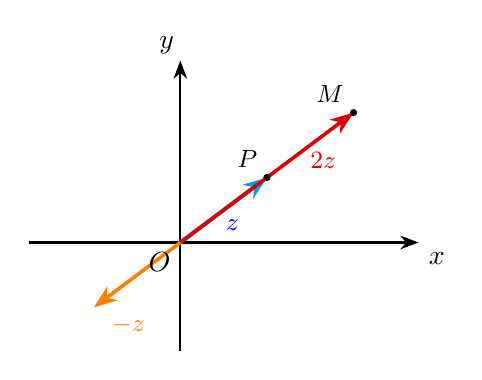
\begin{tikzpicture}[x=0.55cm,y=0.55cm,>=Stealth]
  \coordinate (O) at (0,0);
  \coordinate (P) at (2,1.5);
  \coordinate (M1) at (4,3);   % k=2
  \coordinate (M2) at (-2,-1.5); % k=-1
  \draw[->,line width=0.8pt] (-3.5,0)--(5.5,0) node[below right]{$x$};
  \draw[->,line width=0.8pt] (0,-2.5)--(0,4.2) node[above left=-2pt]{$y$};
  \draw[pptline,line width=1.5pt,-{Stealth[length=3mm,width=2.2mm]}] (O)--(P);
  \draw[pptred,line width=1.3pt,-{Stealth[length=3mm,width=2.2mm]}] (O)--(M1);
  \draw[orange,line width=1.3pt,-{Stealth[length=3mm,width=2.2mm]}] (O)--(M2);
  \fill (P) circle (1.3pt) node[above left] {\small $P$};
  \fill (M1) circle (1.3pt) node[above left] {\small $M$};
  \node[below left] at (O) {$O$};
  \node[pptblue] at (1.2,0.4) {\small $z$};
  \node[pptred] at (3.3,1.9) {\small $2z$};
  \node[orange] at (-1.2,-1.9) {\small $-z$};
\end{tikzpicture}}

% 例4：平行四边形 OACB
\newcommand{\ParallelogramFigure}{%
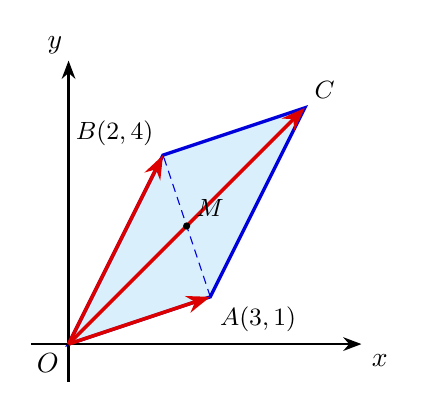
\begin{tikzpicture}[x=0.6cm,y=0.6cm,>=Stealth]
  \coordinate (O) at (0,0);
  \coordinate (A) at (3,1);
  \coordinate (B) at (2,4);
  \coordinate (C) at (5,5);
  \coordinate (M) at (2.5,2.5);
  \fill[pptline!15] (O)--(A)--(C)--(B)--cycle;
  \draw[pptblue,line width=1.2pt] (O)--(A)--(C)--(B)--cycle;
  \draw[densely dashed,pptblue] (O)--(C);
  \draw[densely dashed,pptblue] (A)--(B);
  \draw[->,line width=0.8pt] (-0.8,0)--(6.2,0) node[below right]{$x$};
  \draw[->,line width=0.8pt] (0,-0.8)--(0,6) node[above left=-2pt]{$y$};
  \draw[pptred,line width=1.3pt,-{Stealth[length=3mm,width=2.2mm]}] (O)--(A);
  \draw[pptred,line width=1.3pt,-{Stealth[length=3mm,width=2.2mm]}] (O)--(B);
  \draw[pptred,line width=1.3pt,-{Stealth[length=3mm,width=2.2mm]}] (O)--(C);
  \fill (M) circle (1.3pt);
  \node[below right] at (A) {\small $A(3,1)$};
  \node[above left] at (B) {\small $B(2,4)$};
  \node[above right] at (C) {\small $C$};
  \node[above right] at (M) {\small $M$};
  \node[below left] at (O) {$O$};
\end{tikzpicture}}

% 拓展题图（|z1|=|z2|=1, |z1+z2|=√3）
% 内圆半径1，外圆半径√3。取 z1 在15°、z2 在75°（夹角60°），则 z1+z2 在45°、模√3
\newcommand{\UnitCircleFigure}{%
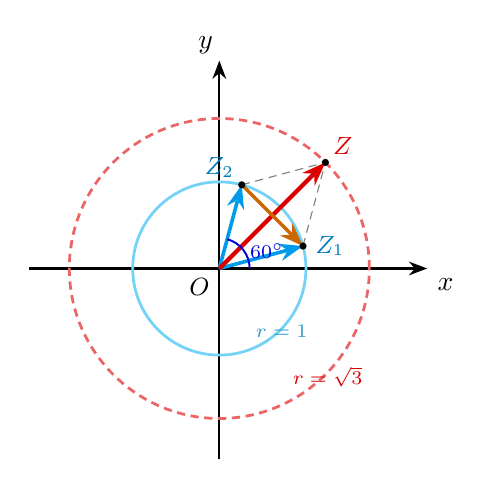
\begin{tikzpicture}[x=1.1cm,y=1.1cm,>=Stealth]
  % 坐标轴
  \draw[->,line width=0.8pt] (-2.2,0)--(2.4,0) node[below right]{$x$};
  \draw[->,line width=0.8pt] (0,-2.2)--(0,2.4) node[above left=-2pt]{$y$};
  % 两个圆
  \draw[cyan!55,line width=1pt] (0,0) circle (1);
  \draw[pptred!60,line width=1pt,densely dashed] (0,0) circle (1.732);
  \node[cyan!80!black,font=\scriptsize] at (0.72,-0.72) {$r=1$};
  \node[pptred,font=\scriptsize] at (1.25,-1.25) {$r=\sqrt{3}$};
  % 关键点（用精确数学关系）
  \coordinate (O) at (0,0);
  \coordinate (Z1) at ({cos(15)},{sin(15)});
  \coordinate (Z2) at ({cos(75)},{sin(75)});
  \coordinate (Z)  at ({1.732*cos(45)},{1.732*sin(45)});
  % 平行四边形虚线
  \draw[densely dashed,gray] (Z1)--(Z);
  \draw[densely dashed,gray] (Z2)--(Z);
  % 三个向量
  \draw[pptline,line width=1.3pt,-{Stealth[length=3mm,width=2.2mm]}] (O)--(Z1);
  \draw[pptline,line width=1.3pt,-{Stealth[length=3mm,width=2.2mm]}] (O)--(Z2);
  \draw[pptred,line width=1.5pt,-{Stealth[length=3mm,width=2.2mm]}] (O)--(Z);
  % z1-z2 虚线（从 Z2 指向 Z1，长度 = 1）
  \draw[orange!80!black,line width=1.2pt,-{Stealth[length=3mm,width=2.2mm]}] (Z2)--(Z1);
  % 标注
  \fill (Z1) circle (1.3pt);
  \fill (Z2) circle (1.3pt);
  \fill (Z)  circle (1.3pt);
  \node[pptline!80!black,right=1pt,font=\small] at (Z1) {$Z_1$};
  \node[pptline!80!black,above left=-1pt,font=\small] at (Z2) {$Z_2$};
  \node[pptred,above right=-1pt,font=\small] at (Z) {$Z$};
  \node[below left,font=\small] at (O) {$O$};
  % 夹角弧
  \draw[pptblue,line width=0.7pt] (0.35,0) arc(0:75:0.35);
  \node[pptblue,font=\scriptsize] at (0.55,0.2) {$60^\circ$};
\end{tikzpicture}}

% 小结思维导图
\newcommand{\SummaryMindMapFigure}{%
\begin{tikzpicture}[x=1cm,y=1cm,>=Stealth,every node/.style={font=\sffamily\small}]
  \tikzset{
    box/.style={draw=pptblue,rounded corners=2pt,fill=pptlightblue,minimum height=0.8cm,inner xsep=4pt},
    smallbox/.style={draw=gray!60,rounded corners=1pt,fill=white,minimum height=0.65cm,inner xsep=4pt},
    conn/.style={draw=pptblue,line width=1pt}
  }
  \node[box,minimum width=3.2cm,align=center,fill=pptpink] (root) at (0,0) {复数的\\ 几何表示};
  \node[box,minimum width=2.6cm] (g1) at (4.5,2.5) {代数表示};
  \node[box,minimum width=2.6cm] (g2) at (4.5,0.8) {几何表示};
  \node[box,minimum width=2.6cm] (g3) at (4.5,-0.9) {模与共轭};
  \node[box,minimum width=2.6cm] (g4) at (4.5,-2.6) {运算几何意义};
  \node[smallbox,minimum width=2.8cm] (g11) at (8.5,2.5) {$z=a+bi$};
  \node[smallbox,minimum width=2.8cm] (g21) at (8.5,1.4) {点 $Z(a,b)$};
  \node[smallbox,minimum width=2.8cm] (g22) at (8.5,0.2) {向量 $\overrightarrow{OZ}$};
  \node[smallbox,minimum width=2.8cm] (g31) at (8.5,-0.4) {$|z|=\sqrt{a^2+b^2}$};
  \node[smallbox,minimum width=2.8cm] (g32) at (8.5,-1.5) {$\overline z = a-bi$};
  \node[smallbox,minimum width=2.8cm] (g41) at (8.5,-2.1) {加减：向量法则};
  \node[smallbox,minimum width=2.8cm] (g42) at (8.5,-3.2) {数乘：伸缩变换};
  \draw[conn] (root.east) .. controls +(1.2,1.0) and +(-1.0,0) .. (g1.west);
  \draw[conn] (root.east) -- (g2.west);
  \draw[conn] (root.east) .. controls +(1.2,-0.3) and +(-1.0,0) .. (g3.west);
  \draw[conn] (root.east) .. controls +(1.2,-1.5) and +(-1.0,0) .. (g4.west);
  \draw[conn] (g1.east) -- (g11.west);
  \draw[conn] (g2.east) -- ++(0.4,0) |- (g21.west);
  \draw[conn] (g2.east) -- ++(0.4,0) |- (g22.west);
  \draw[conn] (g3.east) -- ++(0.4,0) |- (g31.west);
  \draw[conn] (g3.east) -- ++(0.4,0) |- (g32.west);
  \draw[conn] (g4.east) -- ++(0.4,0) |- (g41.west);
  \draw[conn] (g4.east) -- ++(0.4,0) |- (g42.west);
\end{tikzpicture}}



%==================== 新增：图片还原页辅助命令 ====================
\newcommand{\QuestionTitleWithIcon}[1]{%
  \begin{tikzpicture}[x=1cm,y=1cm]
    \node[anchor=west] at (0,0) {\scalebox{1.22}{\QuestionMarkIcon}};
    \node[anchor=west,font=\bfseries\fontsize{18}{23}\selectfont,align=left,text width=11.4cm] at (1.0,0) {#1};
  \end{tikzpicture}\par\vspace{0.18cm}
}

\newcommand{\ChecklistTitleWithIcon}[1]{%
  \begin{tikzpicture}[x=1cm,y=1cm]
    \node[anchor=west] at (0,0) {\scalebox{1.18}{\ChecklistIcon}};
    \node[anchor=west,font=\bfseries\fontsize{20}{25}\selectfont,text=schoolgreen!85!black] at (1.05,0) {#1};
  \end{tikzpicture}\par\vspace{0.2cm}
}

\newcommand{\SummarySquareTitle}[1]{%
  \begin{tikzpicture}[x=1cm,y=1cm]
    \fill[schoolgreen!95!black] (0,0.02) rectangle (0.42,0.44);
    \fill[schoolgreen!90!black] (0.25,-0.16) rectangle (0.58,0.17);
    \node[anchor=west,font=\bfseries\fontsize{20}{25}\selectfont,text=schoolgreen!85!black] at (0.9,0.04) {#1};
  \end{tikzpicture}\par\vspace{0.2cm}
}
%==================== 标题信息 ====================

\title{复数的几何表示}
\subtitle{\S 3.3}
\author{}
\institute{}
\date{}

%==================== 首页命令（带 logo.png 容错） ====================
\newcommand{\makecover}{%
  \begin{frame}[plain]
    \begin{tikzpicture}[remember picture,overlay]
      \fill[white] (current page.south west) rectangle (current page.north east);
      \fill[schoolgreen]
        ([yshift=-2.25cm]current page.north west)
        rectangle
        ([yshift=1.45cm]current page.south east);
      % Logo（如不存在则不加载，避免编译失败）
      \IfFileExists{logo.png}{%
        \node at ([yshift=-1.7cm]current page.north)
          {
\includegraphics[width=3.0cm]{logo.png}};
      }{%
        \node at ([yshift=-1.7cm]current page.north)
          {\color{white}\sffamily\bfseries\fontsize{22}{26}\selectfont 高中数学};
      }
      % 标题
      \node[anchor=center] at ([yshift=-5.65cm]current page.north) {%
        {\fontsize{34}{40}\selectfont\bfseries
          \textcolor{schoolorange}{\S 3.3}\hspace{0.35em}
          \textcolor{white}{复数的几何表示}}%
      };
      % 橙色细线
      \draw[schoolorange,line width=0.9pt]
        ([xshift=-2.65cm,yshift=-6.45cm]current page.north)
        --
        ([xshift= 2.85cm,yshift=-6.45cm]current page.north);
    \end{tikzpicture}
  \end{frame}
}

%==================== 正文 ====================

% 复平面中的点（仅点表示）
\newcommand{\ComplexPointOnlyFigure}{%
	\begin{tikzpicture}[x=0.85cm,y=0.85cm,>=Stealth]
		\draw[->,line width=0.9pt] (-0.3,0)--(4.6,0) node[below]{$x$};
		\draw[->,line width=0.9pt] (0,-0.3)--(0,4.4) node[left]{$y$};
		\coordinate (Z) at (3.2,2.8);
		\draw[densely dashed,pptline!70] (0,2.8)--(Z)--(3.2,0);
		\fill[pptred] (Z) circle (1.8pt) node[above right=-1pt]{$Z$};
		\node[below left] at (0,0) {$O$};
		\node[below] at (3.2,0) {$a$};
		\node[left] at (0,2.8) {$b$};
\end{tikzpicture}}

% 问题页图：复数与平面向量的一一对应
\newcommand{\QuestionFourFigure}{%
	\begin{tikzpicture}[x=0.82cm,y=0.82cm,>=Stealth]
		\draw[rounded corners=0.38cm,draw=schoolgreen!65!black,line width=1.1pt] (0,0) rectangle (12.6,5.3);
		% 左侧坐标图
		\begin{scope}[shift={(0.7,0.8)}]
			\draw[->,line width=0.9pt] (0,0)--(3.5,0) node[below right]{$x$};
			\draw[->,line width=0.9pt] (0,-0.2)--(0,3.5) node[above left=-2pt]{$y$};
			\coordinate (Z) at (2.2,2.2);
			\draw[densely dashed,pptline!70] (0,2.2)--(Z)--(2.2,0);
			\draw[pptred,line width=1.5pt,-{Stealth[length=3mm,width=2.2mm]}] (0,0)--(Z);
			\node[below left] at (0,0) {$O$};
			\node[below] at (2.2,0) {$a$};
			\node[left] at (0,2.2) {$b$};
			\node[above right=-1pt] at (Z) {$Z$};
		\end{scope}
		% 中间两个框
		\node[draw=pptred,rounded corners=0.22cm,line width=0.9pt,minimum width=2.55cm,minimum height=1.5cm,align=center] (A) at (6.2,2.9) {复数\\ $z=a+bi$};
		\node[text=pptred,font=\fontsize{15}{18}\selectfont] at (6.2,1.25) {（数）};
		\node[draw=pptred,rounded corners=0.22cm,line width=0.9pt,minimum width=3.15cm,minimum height=1.5cm,align=center] (B) at (10.0,2.9) {平面向量\\ $\overrightarrow{OZ}=(a,b)$};
		\node[text=pptred,font=\fontsize{15}{18}\selectfont] at (10.0,1.25) {（形）};
		\draw[<->,pptred,line width=1.0pt] (A.east) -- (B.west)
		node[midway,above=3pt,font=\fontsize{15}{18}\selectfont,text=pptred]{一一对应};
\end{tikzpicture}}

% 绿色三圆关系图
\newcommand{\GreenCorrespondenceFigure}{%
	\begin{tikzpicture}[x=0.9cm,y=0.9cm,>=Stealth]
		\colorlet{gc}{schoolgreen!75!black}
		\node[draw=gc,circle,line width=0.9pt,minimum size=2.55cm,align=center] (top) at (0,2.9) {复数\\ $z=a+bi$};
		\node[draw=gc,circle,line width=0.9pt,minimum size=2.55cm,align=center] (left) at (-2.95,-0.15) {平面\\ 内的点\\ $Z(a,b)$};
		\node[draw=gc,circle,line width=0.9pt,minimum size=2.55cm,align=center] (right) at (2.95,-0.15) {平面向量\\ $\overrightarrow{OZ}$};
		\draw[<->,gc,line width=0.95pt] (top.226)--(left.44)
		node[midway,sloped,above=1pt,font=\small,text=gc]{一一对应};
		\draw[<->,gc,line width=0.95pt] (top.314)--(right.136)
		node[midway,sloped,above=1pt,font=\small,text=gc]{一一对应};
		\draw[<->,gc,line width=0.95pt] (left.east)--(right.west)
		node[midway,above=2pt,font=\small,text=gc]{一一对应};
\end{tikzpicture}}

% 标题小图标：问题
\newcommand{\QuestionMarkIcon}{%
	
\begin{tikzpicture}[x=1cm,y=1cm]
		\fill[schoolgreen!80] (0.28,0.18) ellipse (0.22 and 0.18);
		\fill[schoolgreen!80] (0.28,0.57) circle (0.14);
		\fill[schoolgreen!80] (0.58,0.82) circle (0.11);
		\node[text=white,font=\bfseries\scriptsize] at (0.58,0.82) {?};
\end{tikzpicture}}

% 标题小图标：清单
\newcommand{\ChecklistIcon}{%
	
\begin{tikzpicture}[x=1cm,y=1cm,line cap=round,line join=round]
		\draw[schoolgreen!80,line width=1.1pt,rounded corners=0.06cm] (0.10,0.10) rectangle (0.66,0.78);
		\draw[schoolgreen!80,line width=1.1pt] (0.24,0.86) -- (0.52,0.86);
		\draw[schoolgreen!80,line width=1.1pt] (0.22,0.58)--(0.28,0.52)--(0.40,0.66);
		\draw[schoolgreen!80,line width=1.1pt] (0.22,0.38)--(0.28,0.32)--(0.40,0.46);
		\draw[schoolgreen!80,line width=1.1pt] (0.22,0.18)--(0.28,0.12)--(0.40,0.26);
		\draw[schoolgreen!80,line width=1.0pt] (0.46,0.59)--(0.57,0.59);
		\draw[schoolgreen!80,line width=1.0pt] (0.46,0.39)--(0.57,0.39);
		\draw[schoolgreen!80,line width=1.0pt] (0.46,0.19)--(0.57,0.19);
\end{tikzpicture}}

%==================== 正文 ====================
\begin{document}

% ==================== 首页 ====================
\makecover

% ==================== 第2页：问题引入（类比联想） ====================
\begin{frame}[t]
\vspace{0.15cm}

% 顶部标题：绿色小方块装饰 + 标题文字
\begin{tikzpicture}
  \fill[schoolgreen] (0,0) rectangle (0.4,0.4);
  \fill[schoolgreen!60] (0.5,-0.12) rectangle (0.82,0.2);
  \node[anchor=west,font=\bfseries\fontsize{19}{23}\selectfont,text=schoolgreen]
    at (1.1,0.18) {类比联想\ \ 探究新知};
\end{tikzpicture}

\vspace{0.35cm}

% 问题1：无图标版
{\color{pptblue}\bfseries\fontsize{17}{21}\selectfont 问题1\ \ 实数的几何意义是什么？}

\pause
\vspace{0.4cm}

% 中心大圆角框：数形结合
\begin{center}
\begin{tikzpicture}[>=Stealth]
  % 外框
  \draw[schoolgreen!60,rounded corners=10pt,line width=1.2pt,fill=schoolgreen!5]
    (-6.3,-1.9) rectangle (6.3,1.5);

  % 顶部红色文字
  \node[font=\bfseries\fontsize{16}{20}\selectfont,text=pptred]
    at (0,0.95) {实数用数轴上的点来表示};

  % 左侧蓝色框
  \node[draw=pptblue,line width=1pt,rounded corners=4pt,
        minimum width=2.8cm,minimum height=0.9cm,
        font=\fontsize{15}{19}\selectfont] (L) at (-3,-0.35) {实数};
  % 右侧蓝色框
  \node[draw=pptblue,line width=1pt,rounded corners=4pt,
        minimum width=3.4cm,minimum height=0.9cm,
        font=\fontsize{15}{19}\selectfont] (R) at (3,-0.35) {数轴上的点};


\draw[<->,pptblue,line width=1.2pt] (L.east) -- (R.west)
node[midway,above=3pt,inner sep=1pt,font=\small,text=pptblue]{一一对应};

  % 下方红色标注
  \node[font=\bfseries,text=pptred] at (-3,-1.45) {（数）};
  \node[font=\bfseries,text=pptred] at (3,-1.45) {（形）};
\end{tikzpicture}
\end{center}

%\pause
%\vspace{0.15cm}
%\begin{center}
%{\color{pptblue}\bfseries\fontsize{15}{19}\selectfont
%这就是\textcolor{pptred}{数形结合}的思想。}
%\end{center}

\end{frame}

% ==================== 第3页：实数的代数表示（向量） ====================
\begin{frame}[t]
\vspace{0.15cm}
\TopPageTitle{实数的几何表示}

\begin{columns}[T,totalwidth=\textwidth]
\column{0.50\textwidth}
\vspace{0.2cm}
取数轴上一个\textcolor{pptred}{单位向量} $\bm{e}$，则对任意实数 $a$，有
\[
\overrightarrow{OP}=a\bm{e}.
\]

\pause
\vspace{0.15cm}
\begin{calloutbox}
\centering
每一个实数 $a$\\[0.2em]
$\longleftrightarrow$\\[0.2em]
数轴上唯一的向量 $a\bm{e}$
\end{calloutbox}

\pause
\vspace{0.15cm}
{\color{pptblue}\bfseries 过渡}：复数 $z=a+bi$ 呢？能否像实数一样，也找到一个几何对象来表示？

\column{0.45\textwidth}
\vspace{0.3cm}
\begin{center}
{\color{pptred}\bfseries\small 实数的几何表示}\\[0.3cm]
\RealAxisVectorTikz
\end{center}

\end{columns}
\end{frame}

% ==================== 新增：问题2——确定一个复数的要素 ====================
\begin{frame}[t]
\vspace{0.15cm}

\TopPageTitle{问题2\ \ 确定一个复数的要素是什么？}

\pause
\vspace{0.05cm}

% 中心大圆角框
\begin{center}
\begin{tikzpicture}[>=Stealth]
  % 外框
  \draw[schoolgreen!60,rounded corners=10pt,line width=1.2pt,fill=schoolgreen!5]
    (-6.5,-2.8) rectangle (6.5,2.2);

  % 中心公式：z = a + bi (a, b∈ℝ)
  % 将公式分段放置，a 和 b 单独成为 node 便于加框
  \node[font=\fontsize{20}{24}\selectfont] (zeq) at (-3.8,0.6) {$z\ =$};
  \node[draw=pptblue,line width=1pt,rounded corners=2pt,
        inner sep=3pt,font=\fontsize{20}{24}\selectfont] (a) at (-2.6,0.6) {$a$};
  \node[font=\fontsize{20}{24}\selectfont] (plus) at (-1.7,0.6) {$+$};
  \node[draw=pptblue,line width=1pt,rounded corners=2pt,
        inner sep=3pt,font=\fontsize{20}{24}\selectfont] (b) at (-0.9,0.6) {$b$};
  \node[font=\fontsize{20}{24}\selectfont,anchor=west] at (-0.4,0.6) {$i\ (a,b\in\mathbb R)$};

  % 下方"实部""虚部"框（slide 3 出现）
  \onslide<3->{
    \node[draw=pptblue,line width=1pt,rounded corners=4pt,
          minimum width=2.4cm,minimum height=0.85cm,
          font=\fontsize{15}{19}\selectfont] (re) at (-3.5,-1.6) {实部};
    \node[draw=pptblue,line width=1pt,rounded corners=4pt,
          minimum width=2.4cm,minimum height=0.85cm,
          font=\fontsize{15}{19}\selectfont] (im) at (-0.6,-1.6) {虚部};
    % 连接线：a -> 实部，b -> 虚部
    \draw[pptblue,line width=0.9pt] (a.south) -- ++(0,-0.4) -| (re.north);
    \draw[pptblue,line width=0.9pt] (b.south) -- ++(0,-0.4) -| (im.north);
  }

  % 右侧 (a,b) 有序实数对（slide 4 出现）
  \onslide<4->{
    \node[font=\bfseries\fontsize{22}{26}\selectfont,text=pptblue]
      at (3.8,-0.5) {$(a,b)$};
    \node[font=\small,text=pptgray,align=center]
      at (3.8,-1.8) {有序实数对};
  }
\end{tikzpicture}
\end{center}

\pause
\vspace{0.1cm}
\begin{center}
{\color{pptblue}\bfseries\fontsize{14}{18}\selectfont
一个复数 $\longleftrightarrow$ 它的实部和虚部 $\longleftrightarrow$ 有序实数对 $(a,b)$}
\end{center}

\end{frame}

% ==================== 第4页：复数↔有序实数对↔点（5帧动画） ====================
\begin{frame}[t]
\vspace{0.1cm}

\TopPageTitle{问题3\ \ 复数 $z=a+bi$ 的几何表示是什么？}

\vspace{0.05cm}

% 中央大圆角框
\begin{center}
\resizebox{!}{0.75\textheight}{%
\begin{tikzpicture}[>=Stealth]
  % 外框
  \draw[schoolgreen!60,rounded corners=10pt,line width=1.2pt,fill=white]
    (-7,-3.6) rectangle (7,2.8);

  % === 上方蓝色框：有序实数对 ===
  \onslide<1->{
    \node[draw=pptblue,line width=1pt,rounded corners=4pt,
          minimum width=3.5cm,minimum height=1.5cm,align=center,
          font=\fontsize{14}{18}\selectfont] (pair) at (-1.8,1.5) {有序实数对\\ $(a,b)$};
  }

  % === 左下红色框：复数 ===
  \onslide<1->{
    \node[draw=pptred,line width=1pt,rounded corners=4pt,
          minimum width=3.2cm,minimum height=1.5cm,align=center,
          font=\fontsize{14}{18}\selectfont] (z) at (-4.6,-1.8) {复数\\ $z=a+bi$};
  }

  % === 复数 <-> 有序实数对：一一对应（slide 2）===
  \onslide<2->{
    \draw[<->,pptblue,line width=1.1pt] (z.north) -- (pair.south west)
      node[midway,above left=-2pt,font=\small,text=pptblue]{一一对应};
  }

  % === 右侧坐标系图（slide 3）===
  \onslide<3->{
    \begin{scope}[shift={(3.5,1.2)}]
      \draw[->,line width=0.8pt] (-0.3,0)--(2.5,0) node[below]{\small $x$};
      \draw[->,line width=0.8pt] (0,-0.3)--(0,2.2) node[left]{\small $y$};
      \coordinate (Z) at (1.7,1.3);
      \draw[densely dashed,pptblue!60] (0,1.3)--(Z)--(1.7,0);
      \fill[pptred] (Z) circle (1.8pt);
      \node[right=1pt,font=\small] at (Z) {$Z$};
      \node[below left,font=\scriptsize] at (0,0) {$O$};
      \node[below,font=\scriptsize] at (1.7,0) {$a$};
      \node[left,font=\scriptsize] at (0,1.3) {$b$};
    \end{scope}
  }

  % === 右下红色框：平面直角坐标系内的点 ===
  \onslide<3->{
    \node[draw=pptred,line width=1pt,rounded corners=4pt,
          minimum width=4.8cm,minimum height=1.5cm,align=center,
          font=\fontsize{14}{18}\selectfont] (pt) at (2.4,-1.8) {平面直角坐标系内的点\\ $Z(a,b)$};
  }

  % === 有序实数对 <-> 点：一一对应（slide 4）===
  \onslide<4->{
    \draw[<->,pptblue,line width=1.1pt] (pair.south east) -- (pt.north)
      node[midway,above right=-2pt,font=\small,text=pptblue]{一一对应};
  }

  % === 复数 <-> 点：红色一一对应（slide 5）===
  \onslide<5->{
    \draw[<->,pptred,line width=1.3pt] (z.east) -- (pt.west)
      node[midway,above=3pt,inner sep=1.5pt,font=\small,text=pptred]{一一对应};
  }
  
  % === 数/形 标注（slide 5）===
  \onslide<5->{
    \node[font=\bfseries,text=pptred] at (-4.6,-3.2) {（数）};
    \node[font=\bfseries,text=pptred] at (2.4,-3.2) {（形）};
  }
\end{tikzpicture}%
}
\end{center}

\end{frame}


% ==================== 新增：复数集↔复平面动画 ====================
\begin{frame}[t]
\vspace{0.1cm}
\TopPageTitle{动态演示：复数集 $\longleftrightarrow$ 复平面}

\begin{columns}[T,totalwidth=\textwidth]
\column{0.40\textwidth}
\vspace{0.3cm}
\onslide<1->{
每一个复数 $a+bi$，\\[0.2em]
都对应复平面上\\[0.2em]
\textcolor{pptred}{唯一的一个点} $Z(a,b)$。
}

\vspace{0.4cm}
\onslide<3->{%
\begin{center}
\begin{tikzpicture}[>=Stealth]
  \node[draw=pptblue,fill=pptlightblue,rounded corners=3pt,minimum width=3cm,minimum height=0.75cm,font=\bfseries\small] (l) at (0,0) {复数集 $\mathbb C$};
  \node[draw=pptblue,fill=pptlightblue,rounded corners=3pt,minimum width=3cm,minimum height=0.75cm,font=\bfseries\small] (r) at (0,-1.3) {复平面内所有的点};
  \draw[<->,line width=1.1pt,pptblue] (l) -- (r)
    node[midway,above=3pt,fill=white,inner sep=1pt,font=\scriptsize,text=pptblue]{一一对应};
\end{tikzpicture}
\end{center}
}

\vspace{0.15cm}
\onslide<5->{%
\begin{center}
\small 全体复数\\
\textbf{恰好铺满整个复平面}。
\end{center}
}

\column{0.58\textwidth}
\vspace{0.1cm}
\begin{center}
\resizebox{!}{0.7\textheight}{%
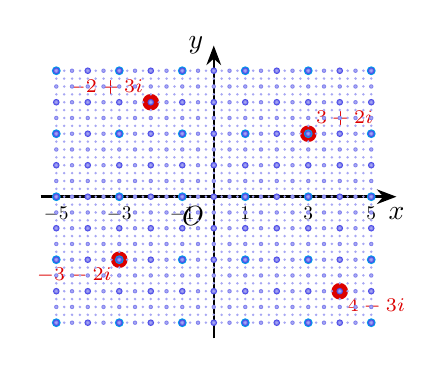
\begin{tikzpicture}[x=0.4cm,y=0.4cm,>=Stealth]
  % 坐标轴
  \draw[->,line width=0.9pt] (-5.5,0)--(5.8,0) node[below]{$x$};
  \draw[->,line width=0.9pt] (0,-4.5)--(0,4.8) node[left]{$y$};
  \node[below left] at (0,0) {$O$};
  \foreach \x in {-5,-3,-1,1,3,5}
    \draw (\x,0.1)--(\x,-0.1) node[below,scale=0.7]{$\x$};

  % slide 1：只有4个"教学用"关键点
  \onslide<1->{
    \foreach \a/\b/\lab/\pos in {3/2/{3+2i}/{above right},
                                  -2/3/{-2+3i}/{above left},
                                  -3/-2/{-3-2i}/{below left},
                                  4/-3/{4-3i}/{below right}}{
      \fill[pptred] (\a,\b) circle (3pt);
      \node[\pos=-1pt,font=\scriptsize,text=pptred] at (\a,\b) {$\lab$};
    }
  }
  % slide 2：加疏格点
  \onslide<2->{
    \foreach \a in {-5,-3,-1,1,3,5}
      \foreach \b in {-4,-2,0,2,4}{
        \fill[pptline] (\a,\b) circle (1.6pt);
      }
  }
  % slide 3：1单位格点
  \onslide<3->{
    \foreach \a in {-5,...,5}
      \foreach \b in {-4,...,4}{
        \fill[pptblue!70] (\a,\b) circle (1.2pt);
      }
  }
  % slide 4：0.5 单位
  \onslide<4->{
    \foreach \a in {-5.0,-4.5,...,5.0}
      \foreach \b in {-4.0,-3.5,...,4.0}{
        \fill[pptblue!50] (\a,\b) circle (0.8pt);
      }
  }
  % slide 5：近似铺满
  \onslide<5->{
    \foreach \a in {-5.00,-4.75,...,5.00}
      \foreach \b in {-4.00,-3.75,...,4.00}{
        \fill[pptblue!35] (\a,\b) circle (0.5pt);
      }
  }
\end{tikzpicture}%
}
\end{center}
\end{columns}
\end{frame}

% ==================== 第5页：复平面定义（文字说明） ====================
\begin{frame}[t]
	\vspace{0.15cm}
	\TopPageTitle{复平面}
	
	\begin{columns}[T,totalwidth=\textwidth]
		\column{0.55\textwidth}
		按上述方式与全体复数建立一一对应关系的平面，叫作\textcolor{pptred}{复平面}。
		
		\pause
		\vspace{0.2cm}
		\begin{itemize}
			\item $x$ 轴叫作\textcolor{pptred}{实轴}
			\item $y$ 轴叫作\textcolor{pptred}{虚轴}
		\end{itemize}
		
		\pause
		\vspace{0.15cm}
		\begin{itemize}
			\item 实轴上的点都表示\textcolor{pptred}{实数}
			\item 除原点外，虚轴上的点都表示\textcolor{pptred}{纯虚数}
		\end{itemize}
		
		\pause
		\column{0.43\textwidth}
		\vspace{0.3cm}
		\begin{center}
			\ComplexPlaneCalloutFigure
		\end{center}
	\end{columns}
\end{frame}


% ==================== 第5页：用向量表示复数 ====================
\begin{frame}[t]
\vspace{0.2cm}
\TopPageTitle{三、复数 $\longleftrightarrow$ 向量}

{\color{pptblue}\sffamily\bfseries\fontsize{17}{21}\selectfont 想一想}\quad 类比实数，复数是否也可以借助平面向量来表示呢？

\pause
\begin{columns}[T,totalwidth=\textwidth]
\column{0.55\textwidth}
\vspace{0.2cm}
设 $\bm{e_1}=(1,0),\ \bm{e_2}=(0,1)$ 为复平面的一组\textcolor{pptred}{基}。对任一向量 $\overrightarrow{OZ}=(a,b)$，有
\[
\overrightarrow{OZ}=a\bm{e_1}+b\bm{e_2}.
\]

\pause
\vspace{0.1cm}
类比实数情形，令 $\bm{e_1}\leftrightarrow 1,\ \bm{e_2}\leftrightarrow i$，则
\[
a\bm{e_1}+b\bm{e_2}\ \longleftrightarrow\ a\cdot 1+b\cdot i=a+bi.
\]

\pause
\vspace{0.15cm}

\begin{center}
\begin{tikzpicture}[>=Stealth]
  % 左框：复数
  \node[draw=pptred,rounded corners=0.22cm,line width=0.9pt,
        minimum width=2.6cm,minimum height=1.35cm,align=center,
        font=\fontsize{13}{16}\selectfont]
        (A) at (0,0) {复数\\ $z=a+bi$};
  % 右框：平面向量
  \node[draw=pptred,rounded corners=0.22cm,line width=0.9pt,
        minimum width=3.2cm,minimum height=1.35cm,align=center,
        font=\fontsize{13}{16}\selectfont]
        (B) at (5.2,0) {平面向量\\ $\overrightarrow{OZ}=(a,b)$};
  % 双向箭头 + "一一对应"标签（文字放在箭头上方，留足间距）
  \draw[<->,pptred,line width=1.0pt] (A.east) -- (B.west)
    node[midway,above=4pt,font=\fontsize{13}{16}\selectfont,text=pptred]{一一对应};
  % "（数）""（形）"标签
  \node[text=pptred,font=\fontsize{12}{15}\selectfont] at (A.south) [below=2pt] {（数）};
  \node[text=pptred,font=\fontsize{12}{15}\selectfont] at (B.south) [below=2pt] {（形）};
\end{tikzpicture}
\end{center}

\column{0.43\textwidth}
\vspace{0.2cm}
\begin{center}
\ComplexVectorFigure
\end{center}
\end{columns}
\end{frame}


% ==================== 新增页：复数的几何意义 ====================
\begin{frame}[t]
	\vspace{0.08cm}
	\noindent
	\begin{minipage}[c]{0.07\textwidth}
		\centering
		\ChecklistIcon
	\end{minipage}%
	\begin{minipage}[c]{0.90\textwidth}
		{\color{schoolgreen!80!black}\bfseries\fontsize{24}{28}\selectfont 复数的几何意义}
	\end{minipage}
	
	\vspace{0.25cm}
	\begin{columns}[T,totalwidth=\textwidth]
		\column{0.24\textwidth}
		\vspace{1.15cm}
		\begin{center}
			\resizebox{!}{0.28\textheight}{\ComplexPointOnlyFigure}
		\end{center}
		
		\column{0.52\textwidth}
		\begin{center}
			\resizebox{!}{0.42\textheight}{\GreenCorrespondenceFigure}
		\end{center}
		
		\column{0.24\textwidth}
		\vspace{1.15cm}
		\begin{center}
			\resizebox{!}{0.28\textheight}{\ComplexVectorFigure}
		\end{center}
	\end{columns}
\end{frame}



% ==================== 第7页：例1题目 ====================
\begin{frame}[t]
\vspace{0.1cm}
\TopPageTitle{例1\ \ 画出复数对应的点}

\begin{columns}[T,totalwidth=\textwidth]
\column{0.54\textwidth}
\vspace{0.05cm}
(1) 在复平面上画出与复数 $z_1,z_2,z_3,z_4$ 对应的点 $P_1,P_2,P_3,P_4$：
\[
z_1=1,\ z_2=i,\ z_3=4+3i,\ z_4=4-3i.
\]

\onslide<6->{\vspace{0.1cm}
(2) 求 $|\overrightarrow{OP_1}|,|\overrightarrow{OP_2}|,|\overrightarrow{OP_3}|,|\overrightarrow{OP_4}|$。}

\onslide<7->{\vspace{0.1cm}
(3) 点 $P_1,P_2,P_3,P_4$ 中是否存在两个点关于实轴对称？若存在，它们对应的复数有什么关系？}

\column{0.44\textwidth}
\vspace{0.2cm}
\begin{center}
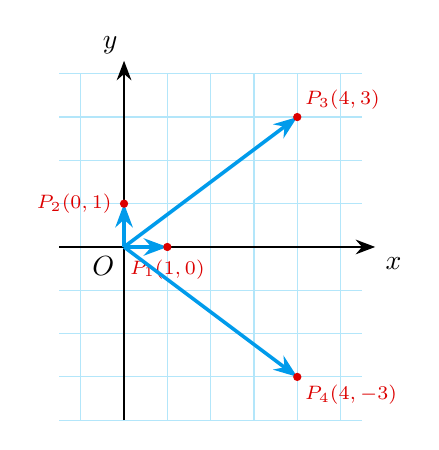
\begin{tikzpicture}[x=0.55cm,y=0.55cm,>=Stealth]
  \draw[step=1,draw=cyan!30,line width=0.4pt] (-1.5,-4) grid (5.5,4);
  \draw[->,line width=0.9pt] (-1.5,0)--(5.8,0) node[below right]{$x$};
  \draw[->,line width=0.9pt] (0,-4)--(0,4.3) node[above left=-2pt]{$y$};
  \node[below left] at (0,0) {$O$};
  % P1 在 slide 2 出现
  \onslide<2->{
    \draw[pptline,line width=1.3pt,-{Stealth[length=3mm,width=2.2mm]}] (0,0)--(1,0);
    \fill[pptred] (1,0) circle (1.5pt);
    \node[pptred,below=1pt,font=\scriptsize] at (1,0) {$P_1(1,0)$};
  }
  % P2 在 slide 3 出现
  \onslide<3->{
    \draw[pptline,line width=1.3pt,-{Stealth[length=3mm,width=2.2mm]}] (0,0)--(0,1);
    \fill[pptred] (0,1) circle (1.5pt);
    \node[pptred,left=1pt,font=\scriptsize] at (0,1) {$P_2(0,1)$};
  }
  % P3 在 slide 4 出现
  \onslide<4->{
    \draw[pptline,line width=1.3pt,-{Stealth[length=3mm,width=2.2mm]}] (0,0)--(4,3);
    \fill[pptred] (4,3) circle (1.5pt);
    \node[pptred,above right=-1pt,font=\scriptsize] at (4,3) {$P_3(4,3)$};
  }
  % P4 在 slide 5 出现
  \onslide<5->{
    \draw[pptline,line width=1.3pt,-{Stealth[length=3mm,width=2.2mm]}] (0,0)--(4,-3);
    \fill[pptred] (4,-3) circle (1.5pt);
    \node[pptred,below right=-1pt,font=\scriptsize] at (4,-3) {$P_4(4,-3)$};
  }
\end{tikzpicture}
\end{center}
\end{columns}
\end{frame}

% ==================== 第8页：例1解答 ====================
\begin{frame}[t]
\vspace{0.2cm}
\TopPageTitle{例1\ \ 解答}

\textbf{(1)} 由复数的几何意义，四点位置如图所示。

\pause
\vspace{0.2cm}
\textbf{(2)} 由 $P_1(1,0),P_2(0,1),P_3(4,3),P_4(4,-3)$，得
\[
|\overrightarrow{OP_1}|=1,\quad |\overrightarrow{OP_2}|=1,
\]
\[
|\overrightarrow{OP_3}|=\sqrt{4^2+3^2}=5,\quad |\overrightarrow{OP_4}|=\sqrt{4^2+(-3)^2}=5.
\]

\pause
\vspace{0.2cm}
\textbf{(3)} 点 $P_3(4,3)$ 与 $P_4(4,-3)$ \textcolor{pptred}{关于实轴对称}，

\pause
它们对应的复数 $4+3i$ 与 $4-3i$：\textcolor{pptred}{实部相同，虚部互为相反数}。

\end{frame}


% ==================== 第12页：问题5——复数的模 ====================
\begin{frame}[t]
\vspace{0.08cm}
\TopPageTitle{问题5\ \ 绝对值 $|a|\ (a\in\mathbb R)$ 能否推广到复数？}

\vspace{0.1cm}
% 实数绝对值示意（居中、小巧）
\begin{center}
{\color{pptblue}\sffamily\bfseries\fontsize{14}{17}\selectfont 回忆：实数\ $a$\ 的绝对值 = 数轴上点 $a$ 到原点 $O$ 的距离}\\[0.15cm]
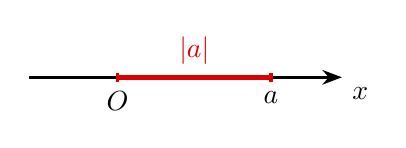
\begin{tikzpicture}[x=0.75cm,y=0.75cm,>=Stealth]
  \draw[->,line width=0.9pt] (-0.3,0)--(5.0,0) node[below right]{$x$};
  \draw[pptred,line width=1.3pt] (1.2,0.08)--(1.2,-0.08);
  \draw[pptred,line width=1.3pt] (3.8,0.08)--(3.8,-0.08);
  \draw[pptred,line width=1.8pt] (1.2,0)--(3.8,0);
  \node[below] at (1.2,-0.08) {$O$};
  \node[below] at (3.8,-0.08) {$a$};
  \node[above,text=pptred] at (2.5,0.05) {$|a|$};
\end{tikzpicture}
\end{center}

\pause
\vspace{0.15cm}
\begin{center}
{\color{pptline}\sffamily\bfseries\fontsize{15}{19}\selectfont 类比推广到复数 $z=a+bi$}
\end{center}

\pause
\vspace{0.1cm}
\begin{calloutbox}
\textbf{定义}\ \ 复数 $z=a+bi$ 所对应的向量 $\overrightarrow{OZ}$ 的\textcolor{pptred}{长度}，叫作复数 $z$ 的\textcolor{pptred}{\bfseries 模}（也称\textbf{绝对值}），记作 $|z|$。
\end{calloutbox}

\pause
\vspace{0.12cm}
\begin{keybox}
\centering
$|z|=|a+bi|=|\overrightarrow{OZ}|=\sqrt{a^2+b^2}$
\end{keybox}

\end{frame}



% ==================== 第11页：例2题目（课本） ====================
\begin{frame}[t]
\vspace{0.2cm}
\TopPageTitle{例2\ \ 点集与圆环}
设 $z\in\mathbb C$，点 $Z$ 对应复数 $z$。求在复平面内满足下列条件的点 $Z$ 的集合是什么图形？

\vspace{0.2cm}
\quad (1) $\modz{z}=2$；\qquad (2) $2\le \modz{z}\le 3$。

\pause
\vspace{0.3cm}
\textbf{解 (1)}\quad $\modz{z}=2$ 表示 $\overrightarrow{OZ}$ 的长度等于 $2$，即点 $Z$ 到原点 $O$ 的距离等于 $2$。

\pause
\vspace{0.1cm}
因此点 $Z$ 的集合是\textcolor{pptred}{以 $O$ 为圆心、$2$ 为半径的圆}。
\end{frame}

% ==================== 第12页：例2（2） ====================
\begin{frame}[t]
\vspace{0.15cm}
\TopPageTitle{例2\ \ 解答（2）}
\textbf{解 (2)}\quad $2\le \modz{z}\le 3$ 可化为不等式组
\[
\begin{cases}\modz{z}\le 3,\\ \modz{z}\ge 2.\end{cases}
\]

\begin{columns}[T,totalwidth=\textwidth]
\column{0.58\textwidth}
\pause
\begin{itemize}
  \item $\modz{z}\le 3$：以 $O$ 为圆心、$3$ 为半径的圆\textbf{及其内部}；
  \pause
  \item $\modz{z}\ge 2$：以 $O$ 为圆心、$2$ 为半径的圆\textbf{及其外部}。
\end{itemize}

\pause
\vspace{0.2cm}
两个集合的\textcolor{pptred}{交集}即所求。

\pause
\vspace{0.15cm}
\begin{keybox}
\centering
以 $O$ 为圆心，半径为 $2$ 和 $3$ 的\\
\textbf{两圆所夹的圆环（含边界）}。
\end{keybox}

\column{0.40\textwidth}
\vspace{0.3cm}
\begin{center}
\resizebox{!}{0.55\textheight}{\AnnulusFigure}
\end{center}
\end{columns}
\end{frame}



% ==================== 第15页：问题6 z²=|z|² 是否成立 ====================
\begin{frame}[t]
\vspace{0.08cm}
\TopPageTitle{问题6\ \ 复数中 $z^2=|z|^2$ 成立吗？}

\vspace{0.15cm}
{\color{pptblue}\sffamily\bfseries\fontsize{15}{19}\selectfont 回忆：}在实数中有 $a^2=|a|^2$，在向量中有 $\vec a^{\,2}=|\vec a|^2$。那么在复数中呢？

\pause
\vspace{0.3cm}
设 $z=a+bi\ (a,b\in\mathbb R)$，分别计算：
\[
z^2=(a+bi)^2=a^2+2abi-b^2,
\]

\pause
\vspace{0.05cm}
\[
|z|^2=\left(\sqrt{a^2+b^2}\right)^2=a^2+b^2.
\]

\pause
\vspace{0.25cm}
\begin{keybox}
\centering
当 $b=0$ 时，$z^2=|z|^2$；\qquad
当 $b\neq 0$ 时，\textcolor{pptred}{$z^2\neq |z|^2$}。
\end{keybox}

\pause
\vspace{0.2cm}
\begin{center}
{\color{pptblue}\small 结论：$z^2=|z|^2$ 不恒成立，仅在 $z$ 为实数时成立。}
\end{center}
\end{frame}


% ==================== 第16页：共轭复数 ====================
\begin{frame}[t]
\vspace{0.08cm}
\TopPageTitle{共轭复数}

\begin{columns}[T,totalwidth=\textwidth]
\column{0.58\textwidth}
\vspace{0.15cm}
对任意复数 $z=a+bi\ (a,b\in\mathbb R)$，保持实部 $a$ 不变，将虚部 $b$ 变为其相反数 $-b$，所得复数 $a-bi$ 称为 $z$ 的\textcolor{pptred}{\bfseries 共轭复数}，记作 $\overline z$，即
\[
\overline{a+bi}=a-bi.
\]

\pause
\vspace{0.1cm}
反过来也有 $\overline{a-bi}=a+bi$，所以
\[
\overline{\overline z}=z.
\]

\pause
\vspace{0.25cm}
\begin{keybox}
\centering
\textbf{几何意义}：复平面内两点关于\textcolor{pptred}{实轴对称}\\[0.2em]
$\Longleftrightarrow$ 它们对应的复数互为共轭。
\end{keybox}

\pause
\vspace{0.2cm}
\begin{center}
{\color{pptblue}\small 共轭复数的模相等：$|\overline z|=|z|$}
\end{center}

\column{0.40\textwidth}
\vspace{0.35cm}
\begin{center}
\resizebox{!}{0.65\textheight}{\ConjugateGridFigure}
\end{center}
\end{columns}
\end{frame}



% ==================== 第17页：问题8 加法的几何意义 ====================
\begin{frame}[t]
\vspace{0.08cm}
\TopPageTitle{问题8\ \ 复数加法 $z_1+z_2$ 的几何意义}

\vspace{0.05cm}
设 $z_1=a+bi,\ z_2=c+di\ (a,b,c,d\in\mathbb R)$，则
\[
z_1+z_2=(a+c)+(b+d)i.
\]

\pause
\vspace{0.1cm}
\begin{columns}[T,totalwidth=\textwidth]
\column{0.55\textwidth}
\vspace{0.3cm}
设 $z_1,z_2,z_1+z_2$ 对应的点分别为 $Z_1,Z_2,Z$，则
\[
\overrightarrow{OZ_1}=(a,b),\ \overrightarrow{OZ_2}=(c,d),
\]
\[
\overrightarrow{OZ}=(a+c,\ b+d).
\]

\pause
\vspace{0.2cm}
\begin{keybox}
\centering
$\overrightarrow{OZ}=\overrightarrow{OZ_1}+\overrightarrow{OZ_2}$\\[0.25em]
\textcolor{pptred}{\bfseries 复数加法 $\Longleftrightarrow$ 向量加法（平行四边形法则）}
\end{keybox}

\column{0.43\textwidth}
\vspace{0.1cm}
\begin{center}
\resizebox{!}{0.58\textheight}{\AdditionFigure}
\end{center}
\end{columns}
\end{frame}



% ==================== 第18页：问题11 减法的几何意义 ====================
\begin{frame}[t]
\vspace{0.08cm}
\TopPageTitle{问题9\ \ $|z_1-z_2|$ 的几何意义}

\vspace{0.05cm}
由复数减法的几何意义：$z_1-z_2$ 对应向量 $\overrightarrow{Z_2Z_1}$。

\pause
\vspace{0.15cm}
\begin{columns}[T,totalwidth=\textwidth]
\column{0.45\textwidth}
\vspace{0.35cm}
设 $z_1,z_2$ 对应点为 $Z_1(a,b),\ Z_2(c,d)$，则
\[
z_1-z_2=(a-c)+(b-d)i,
\]

\pause
\[
|z_1-z_2|=\sqrt{(a-c)^2+(b-d)^2}.
\]

\pause
\vspace{0.2cm}
这恰好是 $Z_1$ 与 $Z_2$ 两点之间的\textcolor{pptred}{\bfseries 距离}。

\column{0.53\textwidth}
\vspace{0.15cm}
\begin{center}
\resizebox{!}{0.48\textheight}{%
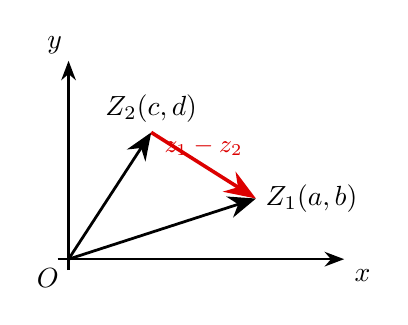
\begin{tikzpicture}[x=0.7cm,y=0.7cm,>=Stealth]
  \draw[->,line width=0.9pt] (-0.2,0)--(5.0,0) node[below right]{$x$};
  \draw[->,line width=0.9pt] (0,-0.2)--(0,3.6) node[above left=-2pt]{$y$};
  \node[below left] at (0,0) {$O$};
  \coordinate (A) at (3.4,1.1);
  \coordinate (B) at (1.5,2.3);
  \draw[line width=1.0pt,-{Stealth[length=3.5mm,width=2.8mm]}] (0,0)--(A);
  \draw[line width=1.0pt,-{Stealth[length=3.5mm,width=2.8mm]}] (0,0)--(B);
  \draw[pptred,line width=1.3pt,-{Stealth[length=4mm,width=3mm]}] (B)--(A);
  \node[anchor=west] at (A) {$Z_1(a,b)$};
  \node[anchor=south] at (B) {$Z_2(c,d)$};
  \node[pptred,above,font=\small] at (2.45,1.7) {$z_1-z_2$};
\end{tikzpicture}}
\end{center}

\pause
\vspace{0.05cm}
\begin{keybox}
\centering
$|z_1-z_2|$ = 两点 $Z_1,\ Z_2$ 间的距离
\end{keybox}
\end{columns}
\end{frame}



% ==================== 第19页：实数与复数相乘（数乘的几何意义）====================
\begin{frame}[t]
\vspace{0.08cm}
\TopPageTitle{实数与复数相乘的几何意义}

\vspace{0.05cm}
设 $z=a+bi$，$k\in\mathbb R$，则
\[
kz=ka+kbi \ \Longrightarrow\ \overrightarrow{OZ'}=(ka,\ kb)=k\,\overrightarrow{OZ}.
\]

\pause
\vspace{0.15cm}
\begin{columns}[T,totalwidth=\textwidth]
\column{0.52\textwidth}
\vspace{0.35cm}
实数 $k$ 与复数 $z$ 相乘的几何意义：\\[0.2em]
将复数 $z$ 对应的向量 $\overrightarrow{OZ}$ 沿 $\overrightarrow{OZ}$ 的方向（或反方向）

\pause
\begin{itemize}
  \item \textbf{放大}：$|k|>1$
  \item \textbf{缩小}：$0<|k|<1$
  \pause
  \item \textbf{反向}：$k<0$
\end{itemize}

\pause
\vspace{0.15cm}
\begin{keybox}
\centering
\textcolor{pptred}{\bfseries 数乘复数 $\Longleftrightarrow$ 向量的伸缩变换}
\end{keybox}

\column{0.45\textwidth}
\vspace{0.2cm}
\begin{center}
\resizebox{!}{0.55\textheight}{\ScalarMulFigure}
\end{center}
\end{columns}
\end{frame}


% ==================== 第17页：例4题目（平行四边形） ====================
\begin{frame}[t]
\vspace{0.15cm}
\TopPageTitle{例4\ \ 平行四边形中的复数运算}

\begin{columns}[T,totalwidth=\textwidth]
\column{0.55\textwidth}
\vspace{0.15cm}
已知复平面上的平行四边形 $OACB$，$O$ 是原点，$A,B$ 分别对应复数
\[
3+i,\quad 2+4i,
\]
$M$ 是 $OC$ 与 $AB$ 的交点。

\pause
\vspace{0.2cm}
求：点 $C$ 与点 $M$ 对应的复数。

\pause
\vspace{0.3cm}
\begin{pinknote}
\textbf{分析}：将几何问题转化为\\
向量的加法与数乘运算。
\end{pinknote}

\column{0.43\textwidth}
\vspace{0.2cm}
\begin{center}
\ParallelogramFigure
\end{center}
\end{columns}
\end{frame}

% ==================== 第18页：例4解答 ====================
\begin{frame}[t]
\vspace{0.2cm}
\TopPageTitle{例4\ \ 解答}

\textbf{求点 $C$：}由 $OACB$ 是平行四边形，
\[
\overrightarrow{OC}=\overrightarrow{OA}+\overrightarrow{OB}.
\]

\pause
\vspace{0.1cm}
由加法的几何意义，$\overrightarrow{OC}$ 对应的复数为
\[
(3+i)+(2+4i)=\textcolor{pptred}{5+5i}.
\]

\pause
\vspace{0.3cm}
\textbf{求点 $M$：}由于 $M$ 是平行四边形对角线的交点，也就是 $OC$ 的中点，
\[
\overrightarrow{OM}=\frac{1}{2}\overrightarrow{OC}.
\]

\pause
\vspace{0.1cm}
由数乘的几何意义，$\overrightarrow{OM}$ 对应的复数为
\[
\frac{1}{2}(5+5i)=\textcolor{pptred}{\frac{5}{2}+\frac{5}{2}i}.
\]
\end{frame}

% ==================== 第19页：拓展题目 + 方法一 ====================
\begin{frame}[t]
\vspace{0.15cm}
\TopPageTitle{能力提升}

{\color{pptblue}\sffamily\bfseries 题目}\quad 已知 $\modz{z_1}=\modz{z_2}=1$，$\modz{z_1+z_2}=\sqrt{3}$，求 $\modz{z_1-z_2}$。

\pause
\vspace{0.1cm}
\begin{columns}[T,totalwidth=\textwidth]
\column{0.55\textwidth}
{\color{pptred}\sffamily\bfseries 方法一（几何法）}

设 $z_1,z_2,z_1+z_2$ 对应点 $Z_1,Z_2,Z$。由题意 $|\overrightarrow{OZ_1}|=|\overrightarrow{OZ_2}|=|\overrightarrow{Z_2Z_1}|=1$，$|\overrightarrow{OZ}|=\sqrt{3}$。

\pause
\vspace{0.1cm}
在 $\triangle OZ_1Z$ 中由余弦定理
\[
3=1+1-2\cos\angle OZ_1Z,
\]

\pause
得 $\cos\angle OZ_1Z=-\tfrac{1}{2}$，$\angle OZ_1Z=120^\circ$。

\pause
于是 $\angle Z_2OZ_1=60^\circ$，$\triangle Z_2OZ_1$ 为\textbf{正三角形}。

\pause
\[
\therefore\ \modz{z_1-z_2}=|\overrightarrow{Z_2Z_1}|=\textcolor{pptred}{1}.
\]

\column{0.43\textwidth}
\begin{center}
\resizebox{!}{0.6\textheight}{\UnitCircleFigure}
\end{center}
\end{columns}
\end{frame}

% ==================== 第20页：拓展题方法二 ====================
\begin{frame}[t]
\vspace{0.15cm}
\TopPageTitle{能力提升\ \ 方法二（代数法）}

设 $z_1=a+bi,\ z_2=c+di\ (a,b,c,d\in\mathbb R)$，由题设得
\[
a^2+b^2=1,\quad c^2+d^2=1,\quad (a+c)^2+(b+d)^2=3.
\]

\pause
\vspace{0.1cm}
展开第三式：
\[
(a+c)^2+(b+d)^2=(a^2+b^2)+(c^2+d^2)+2(ac+bd)=2+2(ac+bd)=3,
\]

\pause
故 $2(ac+bd)=1$。

\pause
\vspace{0.15cm}
于是
\[
\modz{z_1-z_2}^2=(a-c)^2+(b-d)^2=(a^2+b^2)+(c^2+d^2)-2(ac+bd)=2-1=1,
\]

\pause
\[
\therefore\ \modz{z_1-z_2}=\textcolor{pptred}{1}.
\]

\pause
\begin{pinknote}
\centering
\textbf{两种方法对比}：几何法直观简洁，代数法稳健通用。数形结合，相得益彰。
\end{pinknote}
\end{frame}


% ==================== 第24页：小结 ====================
\begin{frame}[t]
\vspace{0.08cm}
\TopPageTitle{小结提升\ \ 形成经验}

\vspace{0.1cm}
\begin{center}
\resizebox{0.88\textwidth}{!}{%
\begin{tikzpicture}[x=0.82cm,y=0.82cm,>=Stealth]
  \draw[rounded corners=0.36cm,draw=schoolgreen!65!black,line width=1.1pt] (0,0) rectangle (13.0,5.8);

  % 左侧：实数→复数
  \node[draw=schoolgreen!30,fill=schoolgreen!10,rounded corners=0.18cm,
        minimum width=4.55cm,minimum height=1.0cm,
        font=\fontsize{18}{24}\selectfont] (topbox) at (3.2,4.55) {实数的几何意义};
  \node[draw=schoolgreen!30,fill=schoolgreen!10,rounded corners=0.18cm,
        minimum width=4.55cm,minimum height=1.0cm,
        font=\fontsize{18}{24}\selectfont] (botbox) at (3.2,1.25) {复数的几何意义};

  \draw[schoolgreen!75,line width=0.18cm,-{Stealth[length=6mm,width=5mm]}] (3.2,3.95)--(3.2,1.95);

  % "类比"标签：放在箭头左侧
  \node[text=schoolorange!85!black,font=\bfseries\fontsize{15}{20}\selectfont,anchor=east] at (2.4,2.95) {类比};
  % "数形结合"标签：放在箭头右侧
  \node[text=schoolorange!85!black,font=\bfseries\fontsize{15}{20}\selectfont,anchor=west,align=left] at (4.0,2.95) {数形\\结合};

  % 右侧：特殊→一般
  \node[draw=schoolorange!70!black,rounded corners=0.16cm,
        minimum width=1.7cm,minimum height=1.0cm,
        font=\bfseries\fontsize{18}{24}\selectfont,text=schoolorange!85!black]
        (spec) at (8.4,4.6) {特殊};
  \node[draw=schoolorange!70!black,rounded corners=0.16cm,
        minimum width=1.7cm,minimum height=1.0cm,
        font=\bfseries\fontsize{18}{24}\selectfont,text=schoolorange!85!black]
        (gene) at (8.4,1.55) {一般};
  \draw[schoolorange!80!black,line width=0.16cm,-{Stealth[length=5.5mm,width=4.5mm]}] (8.4,4.0)--(8.4,2.15);

  % 最右侧：三种素养
  \node[draw=schoolorange!70!black,rounded corners=0.16cm,
        minimum width=1.75cm,minimum height=0.9cm,
        font=\bfseries\fontsize{15}{19}\selectfont,text=schoolorange!85!black,align=center] at (11.0,4.6) {直观\\想象};
  \node[draw=schoolorange!70!black,rounded corners=0.16cm,
        minimum width=1.75cm,minimum height=0.9cm,
        font=\bfseries\fontsize{15}{19}\selectfont,text=schoolorange!85!black,align=center] at (11.0,3.05) {逻辑\\推理};
  \node[draw=schoolorange!70!black,rounded corners=0.16cm,
        minimum width=1.75cm,minimum height=0.9cm,
        font=\bfseries\fontsize{15}{19}\selectfont,text=schoolorange!85!black,align=center] at (11.0,1.5) {数学\\抽象};
\end{tikzpicture}}
\end{center}
\end{frame}



% ==================== 新增页：选做 ====================
\begin{frame}[plain]
\begin{center}
\begin{tikzpicture}[x=0.82cm,y=0.82cm]
  \draw[rounded corners=0.42cm,draw=schoolgreen!50!black,line width=0.9pt,fill=schoolgreen!5] (0,0.35) rectangle (14.0,6.15);
  \fill[schoolgreen!75] (4.5,5.95) rectangle (9.5,7.0);
  \node[text=white,font=\bfseries\fontsize{22}{28}\selectfont] at (7.0,6.47) {选\ 做};
  \node[align=center,text width=12.6cm,font=\fontsize{18}{24}\selectfont] at (7.0,3.7)
  {利用网络画板验证三角不等式：\\[0.7em]
  设 $z_1,z_2\in \mathbb C$，则\\[0.5em]
  $\bigl||z_1|-|z_2|\bigr|\ \leq\ |z_1+z_2|\ \leq\ |z_1|+|z_2|.$};
\end{tikzpicture}
\end{center}
\end{frame}


% ==================== 第22页：结束页 ====================
\begin{frame}[plain]
\begin{tikzpicture}[remember picture,overlay]
  \fill[schoolgreen] (current page.south west) rectangle (current page.north east);
  \node[white,font=\fontsize{36}{42}\selectfont\bfseries] at (current page.center) {谢\ 谢\ 聆\ 听};
  \node[schoolorange,font=\fontsize{18}{22}\selectfont\sffamily]
    at ([yshift=-1.5cm]current page.center) {Thanks for your attention};
\end{tikzpicture}
\end{frame}

\end{document}
